\usepackage{lstmisc}\section{Datenflussanomalieanalyse und abstrakte Interpretation}
Es gitb auch Werkzeuge, die unabhängig von Mustern Fehlersituationen auch anhand der Analyse des Quelltextes erkennen können.\\
Hierzu gibt es zwei Verfahren, die \textbf{Datenflussanomalieanalyse} und die \textbf{abstrakte Interpretation}: Bei beiden Verfahren wird der Zugriff auf Variablen durch mögliche Programmabläufe untersucht (vgl.~\cite[33]{Wed09c}).


\subsection{Datenflussanomalieanalyse}
Die Abfolgen der \textbf{Zugriffe auf Variablen} in den verschiedenen Pfaden eines Kontrollflussgraphen werden bei der \textbf{Datenflussanomalieanalyse} analysiert.\\

\noindent
Zugriffe auf eine Variable werden dazu durch drei Attribute beschrieben (s. Tabelle~\ref{tab:dfaa}):


\begin{table}[]
    \centering
    \setlength{\tabcolsep}{0.5em}
    \def\arraystretch{1.5}
    \begin{tabular}{|c|l|l|}
        \hline
        \textbf{Kürzel} & \textbf{Bedeutung} & \textbf{Beispiel}                                            \\ \hline
        \textbf{d}                                                    & Definition                                                      & \code{x = 5}                                                          \\ \hline
        \textbf{r}                                                    & Referenzierung                                                  & \begin{tabular}[c]{@{}l@{}}\code{y = x + 1}\\ \code{if (x < 4)}\end{tabular} \\ \hline
        \textbf{u}                                                    & Undefinition                                                    & \code{int x;} oder Zerstörung                                         \\ \hline
    \end{tabular}
    \caption{Kürzel in der Datenflussanomalieanalyse und ihre Bedeutung. (Quelle: \cite[33]{VW16c})}
    \label{tab:dfaa}
\end{table}

\noindent
Die Abfolge von Attributen in einem Pfad wird als \textbf{Zugriffssequenz} bezeichnet.

\subsubsection*{Beispiel}

Sei folgendes Beispiel in Java gegeben:

\begin{minted}{java}
    class Pair {
        private int min;
        private int max;

        public void minMax() {
            int hilf;
            if (min > max) {
                max = hilf;
                max = min;
                hilf = min;
            }
        }
    }
\end{minted}

\noindent
\code{minMax()} soll überprüfen, ob \code{min} kleiner als \code{max}, und ansonsten den Inhalt beider vertauschen, was aber im Code nicht umgesetzt ist.
Der Code weist also einen Defekt auf.\\

\noindent
Der Kontrollflussgraph zu \code{minMax} ist in Abbildung~\ref{fig:minmax} gezeigt.

\begin{figure}
    \centering
    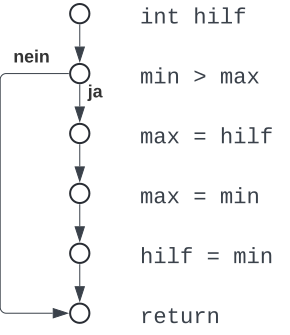
\includegraphics[scale=0.4]{part four/Werkzeuggestützte Analyse/img/minmax}
    \caption{Kontrollflussgraph für \textit{minMax()}. (Quelle: eigene)}
    \label{fig:minmax}
\end{figure}

\noindent
Für die \textit{zwei} möglichen Pfade (\code{min > max} / \code{min <= max}) sind die Zugriffssequenzen der 3 Variablen \code{min}, \code{max} und \code{hilf} in Tabelle~\ref{tab:minmax} aufgelistet.

\begin{table}[]
    \centering
    \setlength{\tabcolsep}{0.5em}
    \def\arraystretch{1.5}
    \begin{tabular}{|c|c|c|}
        \hline
         & \textbf{min > max} & \textbf{min <= max}\\
        \hline
        \code{hilf}                                           & \textbf{urdu}                                          & \textbf{uu}                  \\ \hline
        \code{max}                                            & \textbf{rdd}                                           & \textbf{r}                   \\ \hline
        \code{min}                                            & \textbf{rrr}                                           & \textbf{r}                   \\ \hline
    \end{tabular}
    \caption{Zugriffssequenzen der Variablen für zwei mögliche Pfade in \textit{minMax()}.}
    \label{tab:minmax}
\end{table}

\subsubsection*{3 mögliche Anomalien}
Es gibt bei der Datenflussanomalieanalyse \textbf{3 mögliche Anomalien}, die allesamt in Tabelle~\ref{tab:minmax} auftauchen:

\begin{itemize}
    \item \textbf{ur-Anomalie}: Zugriff auf eine Variable, bevor sie initialisiert wurde.\\
    Der Compiler von Java erkennt diesen Defekt.
    \item \textbf{du-Anomalie}: Definition einer Variable und anschließende Undefinition, ohne, dass auf sie davor lesend / schreibend verwendet wurde
    \item \textbf{dd-Anomalie}: Mehrmalige Definition einer Variable, ohne, dass zwischendurch lesend auf sie zugegriffen wird.
\end{itemize}

\subsubsection*{Anomalie ungleich Defekt}
\textit{Wedemann} stellt fest, dass die \textbf{ur-Anomalie} einen eindeutigen Defekt darstellt, während das bei der \textbf{dd-} bzw. \textbf{du-Anomalie} nicht so ist: Solche Anomalien können u.a. bei Schleifen auftreten (vgl.~\cite[35]{Wed09c}).

\subsubsection*{Schleifen}
Bei Code mit Schleifen ist die Anzahl der möglichen Pfade für eine vollständige Analyse meistens zu groß: Es reicht aber aus, den abweisenden Fall sowie zwei Durchläufe zu analysieren, da bei den Alternativen prinzipiell keine Anomalien hinzukommen können (vgl.~\cite[35]{Wed09c}).

\subsubsection*{Vorgehen}
Das Vorgehen zur Nutzung solcher Werkzeuge entspricht dem Vorgehen bei den bisher beschriebenen werkzeuggestützten Analyse (s. Abschnitt~\ref{sec:programmierrichtlinien}).
Eine sorgfältige Einweisung der Mitarbeiter ist wichtig.

\subsubsection*{Pro und Contra}
\textbf{ur-Anomalien} werden von vielen Compilern entdeckt.
Zur Entdeckung von \textbf{dd-} bzw. \textbf{du-Anomalien} gibt es nicht viele Werkzeuge\footnote{
für Java gibt es beispielsweise das bereits erwähnte \textit{PMD}, s. Abschnitt~\ref{sec:typische-defekte}
}.
Viele Werkzeuge beschränken sich außerdem auf die Analyse von lokalen Variablen und analysieren keine Instanzvariablen, weshalb der Einsatz der Datenflussanomalieanalyse in den meisten Bereichen nur für qualifizierte Entwickler mit einigen Einschränkungen möglich ist (vgl.~\cite[36]{Wed09c}).
Trotz alledem erlaubt die Datenflussanomalianalyse das Auffinden insb. von Defekten in Zusammenhang mit Schleifen, die sonst nur schwer zu entdecken gewesen wären.

\subsection{Abstrakte Interpretation}
Ähnlich wie bei der \textbf{Datenflussanomalieanalyse} wird bei der \textbf{abstrakten Interpretation} bzw. \textbf{abstrakten Semantik} die Nutzung von Variablen in allen Kontrollflüssen analysiert.\\
Es werden hierbei aber keine Kontrollflüsse \textit{konstruiert}, sondern es kommen aufwändige mathematische Verfahren zum Einsatz.

\subsubsection*{Analyse zugewiesener Werte}
Bei der \textbf{abstrakten Interpretation} wird nicht nur die Art der Nutzung von Variablen, sondern auch der Wert, der ihnen zugewiesen wird, analysiert.\\
\textit{Wedemann} gibt hierzu folgendes Beispiel an (vgl.~\cite[36]{Wed09c}):

\begin{minted}{java}
    public void f(int x) {
        if (x < 10) {
            for (int i = 0; i < x; i++) {
                if (i > 10) {
                    // nicht erreichbar
                }
            }
        }
    }
\end{minted}

\noindent
Zeile 5 ist nicht erreichbar:

\begin{enumerate}
    \item nach Zeile 2 is \code{x <= 9}
    \item nach jedem Schleifendurchlauf wird \code{i} um eins erhöht, bis \code{i == x} als Abbruchbedingung erfüllt ist.
    \item[] Da \code{x <= 9} als Voraussetzung gilt, kann also \code{i > 10} niemals erfüllt werden.
\end{enumerate}

\noindent
Analog wird bei der \textbf{abstrakten Interpretation} bspw. auf
\begin{itemize}
    \item die Überschreitung von Array-Grenzen
    \item Overflow bei skalaren Operationen
    \item Division durch 0
    \item Nutzung durch ungültige Zeiger (C / C++)
\end{itemize}
\noindent
geprüft.

\subsubsection*{Beweis der Abwesenheit von Laufzeitfehlern}
Werkzeuge sind auf diese Art und Weise also in der Lage für Quelltext anzugeben, wo prinzipiell keine Laufzeitfehler auftauchen, und wo sie sicher auftauchen werden.\\
Aus diesem Grund ist der Einsatz von solchen Werkzeugen bspw. im Automotive-Bereich vorgeschrieben (vgl.~\cite[36]{Wed09c}).\\
\textit{Wedemann} verweist ebenda auf \textit{Polyspace}\footnote{
\url{https://de.mathworks.com/products/polyspace.html}, abgerufen 24.05.2024
} als verbreitetes Werkzeug zur Analyse von C, C++ und Ada, merkt aber an, dass die Handhabung kompliziert ist und ein spezielles Training benötigt.
